
\section{Galactic Chemical Evolution Models}
\label{outflows:sec:gce}
We use GCE models to shed light on the origin of the disk abundance gradient,
drawing on both one-zone~\citep[e.g.,][]{Tinsley1980, Pagel2009, Matteucci2021}
and multi-zone models~\citep[e.g.,][]{Schoenrich2009a, Minchev2013,
Minchev2014, Chen2023}.
The fundamental assumption of one-zone models is that newly produced metals
mix instantaneously in the star forming ISM.
This approximation sacrifices spatial information in exchange for a reduction
in computational expense, reducing GCE to a system of coupled
integro-differential equations of mass with time.
Multi-zone models add some spatial information back to this framework by
coupling a series of one-zone models via the exchange of gas and stars.
We focus most of our quantitative discussion on our multi-zone models, with our
one-zone models instead providing an analytic framework that is useful for
qualitative interpretation.

% To understand the origin of the disk abundance gradient, we use the multi-ring
% GCE models of Chapter~\ref{migration} and extend them to incorporate radial
% gas flows~\citep[e.g.,][]{Lacey1985, Bilitewski2012}.
% We also extend the analytic framework of~\citet{Weinberg2017b} to incorporate
% the effects of radial gas flows.

% We now construct GCE models to understand the origin of the radial age and
% metallicity gradients characterized in~\S~\ref{outflows:sec:empirical}.
% To this end, we construct models describing the Galaxy disk as a series of
% one-zone models like those in Chapters~\ref{bursts} and~\ref{dga} and
% multi-ring models like those in Chapters~\ref{migration} and~\ref{ohno}.
% Though similar, the former does not incorporate mixing of stellar populations
% while the latter does.
% We also extend these models to incorporate radial gas
% flows~\citep[e.g.,][]{Lacey1985, Bilitewski2012}.
% We present models with numerical solutions predicted by multi-ring GCE models
% of the Galactic disk accounting for both stellar migration and radial flows
% (see~\S~\ref{outflows:sec:gce:multizone}), alongside which we develop an
% analytic framework useful for qualitative interpretation
% (see~\S~\ref{outflows:sec:gce:onezone:analytic}).

\subsection{Multi-Zone Models}
\label{outflows:sec:gce:multizone}

\begin{figure}
\centering
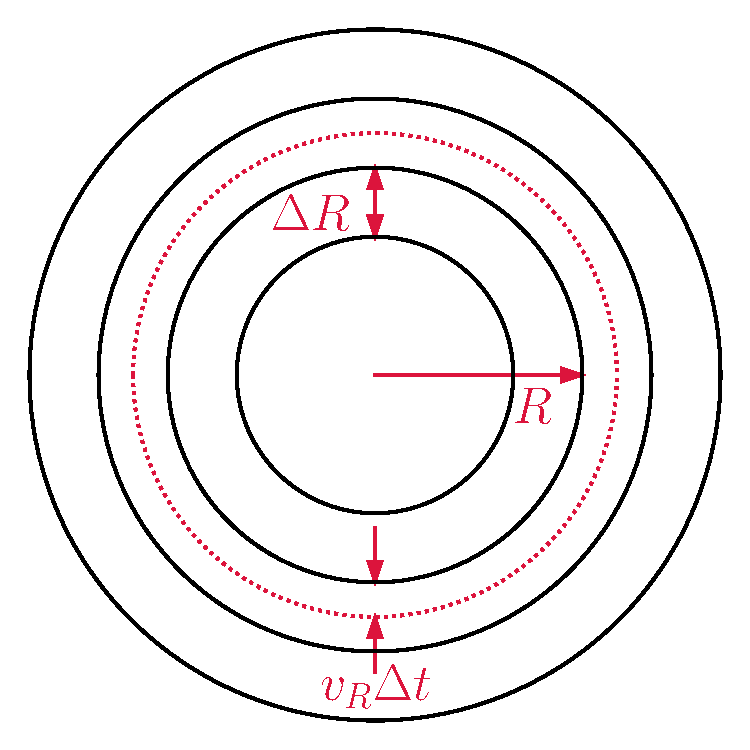
\includegraphics[scale = 0.5]{chapter7/schematic.pdf}
\caption{
A schematic of our multi-ring models illustrating how we handle the flow of gas
between annuli.
At each timestep, the fraction of gas that migrates inward is determined from
the ratio of areas between the [$R$,~$R + v_g \Delta t$) and
[$R$,~$R + \Delta R$) annuli.
}
\label{outflows:fig:schematic}
\end{figure}

Our multi-ring models are adapted from Chapter~\ref{migration}.
We describe the essential details and extensions made for the sake of this
chapter, but otherwise refer to~\S~\ref{migration:sec:methods} for further
details.
A shorter summary of this model can also be found
in~\S~\ref{ohno:sec:multizone}.
\par
First and foremost, we extend these models to incorporate the effects of radial
gas flows.
Fig.~\ref{outflows:fig:schematic} shows a schematic of our parameterization.
A natural consequence of accretion, radial gas flows occur due to the specific
angular momentum of the ISM lowering due to the infalling gas~\citep{Lacey1985,
Bilitewski2012}.
Consequently, each annulus generally experiences a net gain from its outer
neighbor and a net loss to its inner neighbor.
In the limit of a single, characteristic inward flow velocity~$v_g < 0$, all of
the gas in the range [$R$,~$R - v_g \Delta t$) will move in one annulus over
the course of a single~$\Delta t$ timestep.
The ratio of areas between the [$R$,~$R - v_g \Delta t$) and
[$R$,~$R + \Delta R$) annuli then determines the rate of loss due to flows.
The total flow rate, including the rate of gain from an annulus's outer
neighbor, is then given by
\begin{equation}\begin{split}
\dot{M}_{g,\flow} &= M_g(R + \Delta R) \frac{
	v_g(R + \Delta R)^2 \Delta t - 2 (R + \Delta R) v_g
}{
	2 (R + \Delta R) \Delta R + \Delta R^2
} -
\\
&\qquad M_g(R) \frac{
	v_g(R)^2 \Delta t - 2 R v_g
}{
	2 R \Delta R + \Delta R^2
},
\label{outflows:eq:mdot-gas-flow-areafrac}
\end{split}\end{equation}
where we have converted from the change in mass to a rate by dividing by the
timestep size.
The rate of change in the metal mass then follows similarly by multiplying the
gain term by~$Z_x(R + \Delta R)$ and the loss term by~$Z_x(R)$ for a given
element~$x$.
As in previous chapters, we integrate our models with the
\textsc{Versatile Integrator for Chemical Evolution} (\vice; see
Chapter~\ref{bursts}).
\vice~allows users to specify the fractional rate of gas exchange between any
pair of zones, so we simply give it the factors related to the area fraction of
each annulus in equation~\refp{outflows:eq:mdot-gas-flow-areafrac} above.
The effects of the gas moving between rings then arise naturally in its
timestep integrator by simply bookkeeping the changes in mass.
\par
We modify the stellar migration prescription from Chapter~\ref{migration} as
well.
There, we assigned each stellar population in our model an ``analogue'' from
the~\hsim~hydrodynamical simulation~\citep{Christensen2012, Loebman2012,
Loebman2014, Zolotov2012, Brooks2014}.
An analogue is simply a randomly chosen star particle that was born at a
similar radius and time.
Here, we perturb stellar populations from their birth radius by a displacement
randomly sampled from a normal distribution based on arguments in,
e.g.,~\citet{Frankel2018}.
Our model is described in more detail by Dubay et al. (2023, in prep.). 
In short, we fit simple power-laws to the standard deviation of displacement
as a function of radius and age to the~\hsim~star particles.
With a stellar population's sampled orbital displacement in hand, it then
migrates to its implied final radius with a~$\tau^{1/3}$ age dependence as
opposed to the~$\tau^{1/2}$ dependence from Chapter~\ref{migration}.
While we simply took the final midplane distance~$\left|z\right|$ from~\hsim~in
Chapter~\ref{migration}, we randomly sample the midplane distances from
a~$\text{sech}^2(z / 2h_z)$ distribution, where we also fit simple power-laws
to~$h_z$ as a function of radius and age from~\hsim.
\par
We retain the nucleosynthesis prescription of Chapter~\ref{migration}, which
focused on O and Fe, though we adopt different values for the parameters
themselves.
Enrichment of these elements in dominated by SNe~\citep[e.g.,][]{Johnson2019},
and their yields are defined as the net mass of some element~$x$ produced over
all explosion events in the units of the progenitor stellar populations's mass.
For example, a~$1000$~\msun cluster will produce exactly~$1$~\msun~of~$x$ if
the yield~$y_x = 0.001$.
The mass is ejected instantaneously in the case of CCSNe, an approximation
which is valid as long as the relevant timescales of galaxy evolution are
much longer than the lifetimes of massive stars.
In the case of Type Ia supernovae (SNe Ia), the yield is deposited according to
a~$\tau^{-1.1}$ power-law delay-time distribution (DTD) as suggested by
binary population synthesis models~\citep{Greggio2005, Toonen2012,
Maoz2014} and comparisons of the cosmic SFH with volumetric SN Ia rates as a
function of redshift~\citep{Maoz2012a, Maoz2012b, Graur2013, Graur2014}.
We adopt the following values:
\begin{itemize}

	\item \ycc{O} = 0.01

	\item \yia{O} = 0

	\item \ycc{Fe} = 0.0008

	\item \yia{Fe} = 0.0014,

\end{itemize}
which are a factor of~$\sim$$2 / 3$ lower than in Chapter~\ref{migration}.
The original yields are best explained by SN models in which most massive stars
explode, whereas these modifications allow for a portion of massive stars to
collapse directly to black holes~\citep{OConnor2011, Pejcha2015, Gerke2015,
Ertl2016, Sukhbold2016, Adams2017, Basinger2021, Griffith2021b}.
\par
We otherwise retain the same prescriptions as Chapter~\ref{migration}.
The SFH at each radius is normalized such that the predicted surface density
gradient and total stellar mass are consistent with observational estimates
\citep{Bland-Hawthorn2016, Licquia2015}.
The surface densities of star formation and gas are related by a three
component power law, which is steep at intermediate~$\Sigma_g$, based on
\citeauthor{Krumholz2018b}'s~\citeyearpar{Krumholz2018b} compilation of
measurements from~\citet{Bigiel2010} and~\citet{Leroy2013}.
The disk is assumed to be~$13.2$ Gyr old and is discretized into 200 annuli,
each of width 100 pc, with star formation truncating at~$R = 15.5$ kpc.


\subsection{Analytic Framework}
\label{outflows:sec:gce:onezone}
Our analytic framework is an extension of~\citeauthor{Weinberg2017b}
(\citeyear{Weinberg2017b}; hereafter~\citetalias{Weinberg2017b}).
We provide an overview of the essential details and quantities involved here
and refer to their~\S~2 for further details.
Because our main motivation with this framework is qualitative interpretation
of our more complex multi-zone model predictions, we focus the expressions on
O enrichment.
This mathematically simplifies our framework, because O yields are dominated by
massive stars with short lifetimes~\citep[e.g.,][]{Johnson2019}.
This decision enables the approximation that the entire yield is ejected
immediately after a stellar population forms.
Despite the delayed nature of SN Ia enrichment, the predicted abundances of Fe
can be understood from similiar arguments.
\par
In a one-zone model, the rate of change of the ISM mass~$M_g$ is given by a
simple sum of source and sink terms
\begin{equation}\begin{split}
\dot{M}_g &= \dot{M}_\text{in} - \dot{M}_\star - \dot{M}_\text{out} +
\dot{M}_r
\\
&\approx \dot{M}_\text{in} - \dot{M}_\star(1 + \eta - r),
\label{outflows:eq:mdot-gas-noflow}
\end{split}\end{equation}
where~$\dot{M}_\text{in}$ is the accretion rate,~$\dot{M}_\star$ is the SFR,
$\dot{M}_\text{out} \equiv \eta \dot{M}_\star$ is the outflow rate, and
$\dot{M}_r \approx r\dot{M}_\star$ is the return rate of recycled stellar
envelopes to the ISM.
Though the recycling rate in detail is a complex function of age (see
discussion in~\S~\ref{bursts:sec:crf}), it is sufficiently accurate for the
sake of analytic approximations to assume a constant value ($r \approx 4$ for
a~\citealt{Kroupa2001} IMF; see~\S~2 of~\citetalias{Weinberg2017b}).
As discussed in~\S~\ref{outflows:sec:intro}, the mass loading factor~$\eta$ is
of central interest to this chapter, namely in comparing model predictions
with~$\eta > 0$ and~$\eta = 0$.
\par
The rate of O production follows similarly, with the modification that the
source term describes massive star enrichment and the sink term must account
for the abundance by mass~$Z_\text{O} = M_\text{O} / M_g$:
\begin{equation}
\dot{M}_\text{O} = \ycc{O} \dot{M}_\star - Z_\text{O} \dot{M}_\star
\left(1 + \eta - r\right),
\label{outflows:eq:mdot-element-noflow}
\end{equation}
where~$\ycc{O}$ is the IMF-averaged yield of O from CCSNe.
The change in the O abundance~$\dot{Z}_\text{O}$ then follows:
\begin{equation}
\dot{Z}_\text{O} = \ycc{O}\tau_\star^{-1} - Z_\text{O} \tau_\star^{-1}
\left(1 + \eta - r + \tau_\star (\ddot{M}_\star / \dot{M}_\star) \right),
\label{outflows:eq:zdot-noflow}
\end{equation}
where~$\tau_\star \equiv M_g / \dot{M}_\star$ is the star formation efficiency
(SFE) timescale, with low values indicating efficient star formation.
\par
This above expression is a linear ordinary differential equation that can
be solved for a given choice of SFH~$\dot{M}_\star$.
Generally, the predicted metal abundances evolve toward an equilibrium in
which their source and sink terms balance~\citep[see also][]{Larson1974}.
In the case of exponential~$\dot{M}_\star \propto e^{-t / \timescale{sfh}}$
and linear-exponential~$\dot{M}_\star \propto t e^{-t / \timescale{sfh}}$ SFHs,
the equilibrium is given by
\begin{equation}
Z_\text{O,eq} = \frac{\ycc{O}}{1 + \eta - r - \tau_\star / \timescale{sfh}},
\label{outflows:eq:zo-eq-noflow}
\end{equation}
but the detailed evolution toward equilibrium differs based on the SFH.
\par
The primary feature of this extension of the~\citetalias{Weinberg2017b}
framework is a parameterization of radial gas flows appropriate for one-zone
models.
In our multi-zone models, their effects arise by simply exchanging gas between
neighboring annuli under the assumption of a single, uniform flow velocity (see
discussion in~\S~\ref{outflows:sec:gce:multizone} above).
However, we demonstrate in Appendix~\ref{outflows:sec:coefficients-derivation}
that the flow rates have mathematically well defined forms in the limit that
the ring width~$\Delta R$ and timestep size~$\Delta t$ approach zero.
The effects can be understood by introducing the unitless coefficients
$\gamma_\flow$ and~$\mu_\flow$, defined such that the flow rates of
gas and metals is given by
\begin{subequations}\begin{align}
\dot{M}_{g,\flow} &= \dot{M}_\star \gamma_\flow
\label{outflows:eq:mdot-gas-flow}
\\
\dot{M}_\text{O,flow} &= Z_\text{O} \dot{M}_\star \muflow{O}.
\label{outflows:eq:mdot-element-flow}
\end{align}\end{subequations}
These coefficients in a generalized form are given by
\begin{subequations}\begin{align}
\gamma_\flow &\equiv -\tau_\star v_g \left[
\frac{1}{R} +
\frac{\partial \ln \Sigma_g}{\partial R} +
\frac{\partial \ln v_g}{\partial R}
\right]
\label{outflows:eq:gamma-flow-general}
\\
\muflow{O} &\equiv \gamma_\flow - \tau_\star v_g
\frac{\partial \ln Z_\text{O}}{\partial R}
\label{outflows:eq:mu-flow-general}
\end{align}\end{subequations}
where~$\Sigma_g$ is the surface density of the ISM.
$\mu_\flow$ in principle should vary element to element, as indicated by the
dependence on~$Z_\text{O}$ in the above expression.
We reserve detailed derivations of~$\gamma_\flow$ and~$\mu_\flow$ for
Appendix~\ref{outflows:sec:coefficients-derivation}, providing only
qualitative justification of their functional forms here.
\par
The linear dependence on~$\tau_\star$ arises because these rates are tied to
the local gas supply.
When multiplied by the SFR in equations~\refp{outflows:eq:mdot-gas-flow}
and~\refp{outflows:eq:mdot-element-flow},~$\dot{M}_\star \tau_\star$ becomes
$M_g$.
The dependence on both the velocity~$v_g$ and the velocity profile
$\partial \ln v_g / \partial R$ are expected as the rates will naturally change
if gas speeds up or slows down as a function of radius, time, or both.
Both coefficients depend on fluctuations in the ISM surface density since any
changes thereof will affect how much gas is exchanged between neighboring
annuli.
For an inward flow, any given annulus will be replenished with less gas from
its outer neighbor in cases where~$\Sigma_g$ declines steeply with radius.
The metal flow coefficient~$\mu_\flow$ depends on the abundance gradient for a
similar reason.
The explicit~$1 / R$ dependence on radius encodes the ``pile-up'' of material
near the Galactic center as the infalling material converges.
\par
In principle, both of these flow coefficients can vary with time as a
consequence of changes in any one of the parameters they depend on.
However, extending the~\citetalias{Weinberg2017b} framework to include them is
straightforward if they are held constant.
In this limit, one need only apply the simple transformations
$1 + \eta - r \rightarrow \mu_\flow$ for metals and
$1 + \eta - r \rightarrow \gamma_\flow$ for gas.
Equations~\refp{outflows:eq:mdot-gas-noflow},
\refp{outflows:eq:mdot-element-noflow},~\refp{outflows:eq:zdot-noflow},
and~\refp{outflows:eq:zo-eq-noflow} then become
\begin{subequations}\begin{align}
\dot{M}_g &\rightarrow \dot{M}_\text{in} - \dot{M}_\star
\left(1 + \eta - r - \gamma_\flow\right)
\label{outflows:eq:mdot-gas}
\\
\dot{M}_\text{O} &\rightarrow \ycc{O} \dot{M}_\star - Z_\text{O} \dot{M}_\star
\left(1 + \eta - r - \muflow{O}\right)
\label{outflows:eq:mdot-element}
\\
\dot{Z}_\text{O} &\rightarrow \ycc{O} \tau_\star^{-1} -
Z_\text{O} \tau_\star^{-1}
\left(
1 + \eta - r - \muflow{O} + \tau_\star (\ddot{M}_\star / \dot{M}_\star)
\right)
\label{outflows:eq:zdot}
\\
Z_\text{O,eq} &\rightarrow \frac{\ycc{O}}{
	1 + \eta - r - \muflow{O} - \tau_\star / \timescale{sfh}
}.
\label{outflows:eq:zo-eq}
\end{align}\end{subequations}
Enrichment rates and equilibrium abundances depend on~$\mu_\flow$ rather
than~$\gamma_\flow$ because one must account for the effect of the radial
abundance gradient on the metal flow rate.\footnote{
	This realization can be justified mathematically by differentiating
	$Z_\text{O} \equiv M_\text{O} / (\dot{M}_\star \tau_\star)$ with time
	assuming constant~$\tau_\star$ as in~\citetalias{Weinberg2017b}.
}
We describe a handful of cases that offer analytic solutions to the full
time evolution of~$Z_\text{O}$ below before turning to our multi-zone models
in~\S~\ref{outflows:sec:results}.

\subsubsection{Full Time Evolution for Simple Cases}
\label{outflows:sec:gce:onezone:simple-cases}

{
\renewcommand{\arraystretch}{1.8}
\begin{table*}
\caption{
The SFHs we use in this analytic framework (left) and the implied functions of
time specifying the evolution toward chemical equilibrium (right; see equations
\ref{outflows:eq:zo-eq} and~\ref{outflows:eq:f-sfh-definition} and associated
discussion in~\S~\ref{outflows:sec:gce:onezone:simple-cases}).
}
\begin{tabularx}{\linewidth}{l @{\extracolsep{\fill}} r}
\hline
SFH Shape & $f_\text{sfh}$
\\
\hline
$e^{-t / \timescale{sfh}}$ &
$1 - e^{-t / \taupsi{O}}$
\\
$te^{-t / \timescale{sfh}}$ &
$1 - \ddfrac{\taupsi{O}}{t} \left(1 - e^{-t / \taupsi{O}}\right)$
\\
$\left(1 - e^{-t / \timescale{rise}}\right) e^{-t / \timescale{sfh}}$ &
$\ddfrac{1}{1 - e^{-t / \timescale{rise}}} \left(
1 - e^{-t / \taupsi{O}} -
\ddfrac{\timescale{rise}}{\timescale{rise} - \taupsi{O}}
\left(e^{-t / \timescale{rise}} - e^{-t / \taupsi{O}}\right)
\right)$
\\
\hline
\end{tabularx}
\label{outflows:tab:f-sfh-forms}
\end{table*}
}

For both exponential~$\dot{M}_\star \propto e^{-t / \timescale{sfh}}$ and
linear-exponential~$\dot{M}_\star \propto t e^{-t / \timescale{sfh}}$ SFHs,
the equilibrium abundance is the same (given by
equation~\ref{outflows:eq:zo-eq}), but the evolution to equilibrium differs.
$Z_\text{O}(t)$ can then be expressed generally as
\begin{equation}
Z_\text{O}(t) = Z_\text{O,eq} f_\text{sfh}(t),
\label{outflows:eq:f-sfh-definition}
\end{equation}
where~$f_\text{sfh}$ is some unitless function whose form depends on the
choice of~$\dot{M}_\star$.
The functional forms implied by the exponential and linear-exponential SFHs
are listed in Table~\ref{outflows:tab:f-sfh-forms}, where the timescale
$\taupsi{O}$ is given by
\begin{equation}
\taupsi{O} = \left(
\frac{1 + \eta - r - \muflow{O}}{\tau_\star} - \frac{1}{\timescale{sfh}}
\right)^{-1}.
\label{outflows:eq:tau-psi-definition}
\end{equation}
We also derive the expression for~$f_\text{sfh}$ given the ``inside-out'' SFH
from Chapter~\ref{migration}:
\begin{equation}
\dot{M}_\star \propto \left(1 - e^{-t / \timescale{ries}}\right)
e^{-t / \timescale{sfh}}.
\label{outflows:eq:inside-out-sfh}
\end{equation}
The advantage of this parameterization over the simpler linear-exponential form
is the~\timescale{rise}~allows one to adjust how long the SFR is rising at
early times independent of~\timescale{sfh}.
The solution, also noted in Table~\ref{outflows:tab:f-sfh-forms}, follows by
solving equation~\refp{outflows:eq:zdot-noflow} with the proper form
of~$\ddot{M}_\star / \dot{M}_\star$ and then applying the transformation
$1 + \eta - r \rightarrow 1 + \eta - r - \muflow{O}$.





% The main consideration required in transforming the full time evolution of
% $Z_\text{O}$ from~\citetalias{Weinberg2017b} arises because
% $\mu_\flow \neq \gamma_\flow$ unless the metallicity gradient is flat.
% The gas an annulus gains from its outer neighbor will always be lower
% metallicity than its own ISM if the radial gradient is negative, resulting in
% dilution (see discussion in~\S~{\color{red} X} below).
% Quantitatively, the~\textit{depletion time} of metals is shorter than that
% of the bulk ISM:
% \begin{subequations}\begin{align}
% \tau_\text{dep,g} &= \frac{\tau_\star}{
% 	1 + \eta - r - \gamma_\flow
% }
% \\
% \tau_\text{dep,O} &= \frac{\tau_\star}{
% 	1 + \eta - r - \muflow{O}
% }.
% \end{align}\end{subequations}
% These timescales quantify the average amount of time an ISM fluid element
% remains present before being incoporporated into new stars, ejected, or lost to
% a radial flow, and the latter affects metals disproportionately.
% \par
% For both exponential~$\dot{M}_\star \propto e^{-t / \timescale{sfh}}$ and
% linaer-exponential~$\dot{M}_\star \propto t e^{-t / \timescale{sfh}}$ SFHs,
% the equilibrium abundance is the same (given by
% equation~\ref{outflows:eq:zo-eq}), but the evolution to equilibrium differs.
% $Z_\text{O}(t)$


% Enrichment rates depend on the metal depletion time (see
% Appendix~\ref{outflows:sec:coefficients-derivation}), which can vary element
% to element as a consequence of~$\mu_\flow$.
% For both exponential~$\dot{M}_\star \propto e^{-t / \timescale{sfh}}$ and
% linaer-exponential~$\dot{M}_\star \propto t e^{-t / \timescale{sfh}}$ SFHs,
% the equilibrium abundance is the same (given by
% equation~\ref{outflows:eq:zo-eq}), but how it reaches that equilibrium differs.
% $Z_\text{O}(t)$ can then be expressed generally as
% \begin{equation}
% Z_\text{O}(t) = Z_\text{O,eq} f_\text{sfh}(t),
% \label{outflows:eq:f-sfh-definition}
% \end{equation}
% where~$f_\text{sfh}$ is some unitless function of time whose form depends on
% the SFH.
% \par
% The forms of~$f_\text{sfh}$ for these SFHs are given in
% Table~\ref{outflows:tab:f-sfh-forms}, where the timescale~$\taupsi{O}$ is
% defined as
% \begin{equation}
% \taupsi{O} = \left(
% \frac{1 + \eta - r - \muflow{O}}{\tau_\star} - \frac{1}{\timescale{sfh}}
% \right)^{-1}.
% \end{equation}
% We also derive the form of~$f_\text{sfh}$ for the ``inside-out'' SFH from
% Chapter~\ref{migration}, given by
% \begin{equation}
% \dot{M}_\star \propto \left(1 - e^{-t / \timescale{rise}}\right)
% e^{-t / \timescale{sfh}}.
% \end{equation}
% The advantage of this parameterization over the simpler linear-exponential SFH
% is that~$\timescale{rise}$ allows one to adjust how long the SFH is rising at
% early times independent from~$\timescale{sfh}$.
% The solution, given in Table~\ref{outflows:tab:f-sfh-forms} as well, follows by
% solving equation~\refp{outflows:eq:zdot-noflow} with the proper form
% of~$\ddot{M}_\star / \dot{M}_\star$ and then applying the transformation.
% We omit the full derivation of this expression as it is rather verbose.






















% \subsection{Old Text of This Section}


% Because we are primarily interested in this analytic framework for qualitative
% interpretation, we focus on O
% \par
% As discussed in~\S~\ref{outflows:sec:intro}, the ``mass loading factor''
% $\eta$ is of central interest to this chapter.
% This coefficient quantifies how much ambient ISM is swept up and ejected with
% an outflow due to massive star and SN feedback.
% The value of~$\eta$ sets the equilibrium abundance at which metal losses to
% outflows is balanced by production by new stars~\citep[see also][]{Larson1974}.
% A general expression for the equilibrium abundance, which is accurate up to a
% small correction factor for a specific element's delay time distribution (DTD),
% is given by
% \begin{equation}
% Z_{x,\eq} = \frac{y_x}{1 + \eta - r - \tau_\star / \tau_\text{sfh}},
% \label{outflows:eq:zx-eq}
% \end{equation}
% where~\timescale{sfh}~is the e-folding timescale of an exponential SFH,
% and~$\tau_\star \equiv \dot{M}_\star / M_g$ is the inverse of the star
% formation efficiency (SFE).
% The SFE timescale is often referred to as the ``depletion time'' in the
% observational literature on star formation in galaxies, but we retain this
% nomencature as the depletion time of the ISM in these models can be
% significantly shorter than~$\tau_\star$ in the presence of outflows (see
% discussion below).
% \par
% In Chapter~\ref{migration}, we set the value of~$\eta$ as a function of radius
% so that a realistic abundance gradient arose as a consequence of variations in
% the equilibrium abundance.
% Specifically, for a constant SFH (i.e.,~$\timescale{sfh} \rightarrow \infty$),
% it follows from equation~\refp{outflows:eq:zx-eq} that
% \begin{equation}
% \eta = \frac{y_x}{Z_{x,\odot}}
% e^{(R - R_\odot) / R_x} + r - 1,
% \end{equation}
% where~$R_x = -(\grad{X} \ln 10)^{-1}$ is the scale radius required for a
% gradient slope~\grad{X}.
% In this scenario for the abundance gradient, the slope is~\textit{input} to the
% model as opposed to a prediction, though it can be impacted by, e.g., stellar
% migration, radial gas flows, and variations with~$\tau_\star$
% and~\timescale{sfh} with radius.
% A primary focus of this chapter is in the comparison of this scenario with
% models in which~$\eta = 0$ everywhere.
% \par
% {\color{red} (stopped edits here)} In the present chapter, we focus on the
% abundances of alpha and
% iron-peak elements whose production is dominated by SNe
% \citep[e.g.,][]{Johnson2019}.
% We take O and Fe as the prototypical elements from these categories, though
% we expect our GCE models to make similar predictions if we chose different
% elements to compute abundances for.
% The rate of change of the mass of some element~$x$ in the ISM can be
% expressed as
% \begin{equation}
% \dot{M}_x = \ycc{$x$} \dot{M}_\star +
% \yia{$x$} \langle \dot{M}_\star \rangle_\text{Ia} -
% Z_x \dot{M}_\star \left(1 + \eta - r\right),
% % \label{outflows:eq:mdot-element-noflow}
% \end{equation}
% where~$Z_x$ is the abundance by mass of~$x$ in the ISM at a given moment in
% time and~\ycc{$x$} and~\yia{$x$} are the population-averaged yields of~$x$
% from core collapse supernovae (CCSNe) and Type Ia supernovae (SNe Ia),
% respectively.
% This parameterization assumes that all CCSNe yields are ejected immediately
% following a stellar population's formation, which is valid as long as the
% timescales of Galaxy evolution are significantly longer than the lifetimes
% of massive stars.
% Enrichment by SNe Ia is instead weighted by a delay-time distribution (DTD),
% for which we retain the~$t^{-1.1}$ formalism from previous chapters as
% suggested by comparisons of the cosmic SFH~\citep[e.g.,][]{Madau2017,
% Driver2018} with volumetric SN Ia rates as a function of
% redshift~\citep{Maoz2012a, Maoz2012b, Graur2013, Graur2014}.
% \par
% \citet{Weinberg2017b} demonstrate that the first-order details of the
% enrichment history of alpha and iron-peak elements are established by
% the mass-loading factor~$\eta$ and the star formation efficiency (SFE)
% timescale~$\tau_\star \equiv M_g / \dot{M}_\star$ relating the
% gas supply and the star formation rate (SFR).
% The SFE timescale sets the position of the ``knee'' in the~\afe-\feh~plane,
% while~$\eta$ controls the equilibrium abundance at which enrichment is
% balanced by losses to outflows, which sets the end-point of the track.
% The detailed form of the SFH has little impact, instead influencing how
% stars distribute themselves along the track.
% However, the detailed SFH has much more impact on the abundance evolution
% in the~$\eta = 0$ scenario.
% In this case, radial gas flows~\citep[e.g.,][]{Lacey1985}
% also have a much stronger effect since the substantial sink term of
% outflows is removed.
% \par
% To this end, we construct a parameterization for including the effects of
% radial gas flows in one-zone GCE models.
% We introduce the unitless coefficients~$\gamma_\flow$ and~$\mu_\text{flow}$
% defined such that the rates of change of the gas supply and an element~$x$ due
% to flows can be expressed in terms of the SFR and~$Z_x$ according to
% \begin{subequations}\begin{align}
% \dot{M}_{g,\flow} &= \dot{M}_\star \gamma_\flow
% % \label{outflows:eq:mdot-gas-flow}
% \\
% \dot{M}_{x,\flow} &= Z_x \dot{M}_\star \mu_\flow.
% % \label{outflows:eq:mdot-element-flow}
% \end{align}\end{subequations}
% Equations~\refp{outflows:eq:mdot-gas-noflow}
% and~\refp{outflows:eq:mdot-element-noflow} then become
% \begin{subequations}\begin{align}
% \dot{M}_{g} &\rightarrow \dot{M}_\text{in} - \dot{M}_\star
% \left(1 + \eta - r - \gamma_\flow\right)
% \\
% \dot{M}_x &\rightarrow \ycc{$x$} \dot{M}_\star +
% \yia{$x$} \langle \dot{M}_\star \rangle_\text{Ia} -
% Z_x \dot{M}_\star \left(1 + \eta - r - \mu_\flow\right).
% \end{align}\end{subequations}
% The most general forms of these flow coefficients are given by
% \begin{subequations}\begin{align}
% \gamma_\flow &\equiv -\tau_\star v_g \left[
% \frac{1}{R} +
% \frac{\partial \ln \Sigma_g}{\partial R} +
% \frac{\partial \ln v_g}{\partial R}
% \right]
% % \label{outflows:eq:gamma-flow-general}
% \\
% \mu_\flow &\equiv -\tau_\star v_g \left[
% \frac{1}{R} + \frac{\partial \ln \Sigma_g}{\partial R} +
% \frac{\partial \ln v_g}{\partial R} +
% \frac{\partial \ln Z_x}{\partial R}
% \right],
% % \label{outflows:eq:mu-flow-general}
% \end{align}\end{subequations}
% where~$v_g$ is the radial velocity of the ISM gas and~$\Sigma_g$ is its surface
% density.
% Though the ISM in nature has a distribution of radial velocities, this
% parameterization assumes a single characteristic velocity at a given radius.
% The bulk flow is generally directed inward (i.e.,~$v_g < 0$; hence the minus
% signs), which arises due to the angular momentum of the disk being diluted by
% freshly accreted material and falling toward the Galactic center
% \citep[see discussion in, e.g.,][]{Bilitewski2012}.
% These equalities should hold even when each of the quantities are allowed to be
% arbitrary, continuous functions of time, but they are only as accurate as the
% assumptions outlined in Appendix~\ref{outflows:sec:coefficients-derivation}.
% We reserve detailed derivations of~$\gamma_\flow$ and~$\mu_\flow$ for
% Appendix~\ref{outflows:sec:coefficients-derivation}, providing only
% qualitative justification of their functional forms here.
% \par
% The linear dependence on~$v_g$ is expected.
% As the flow velocity increases, its effect on enrichment rates and the gas
% supply increases proportionally.
% The dependence on the velocity profile is also intuitive.
% For example, if the radial velocity slows as it falls due to, e.g., mixing with
% higher density ISM on a less eccentric orbit, then its possible for material to
% enter an annulus faster than it is leaving, leading to a ``pile-up.''
% The linear dependence on~$\tau_\star$ arises because these rates are tied to
% the local gas supply.
% When multiplied by the SFR in equations~\refp{outflows:eq:mdot-gas-flow}
% and~\refp{outflows:eq:mdot-element-flow},~$\dot{M}_\star \tau_\star$ becomes
% $M_g$ by definition.
% Both coefficients depend on fluctuations in the ISM surface density since any
% variation thereof will affect how much gas is exchanged between neighboring
% annuli.
% The metal flow coefficient~$\mu_\flow$ additionally depends on the abundance
% gradient for similar reasons.
% For an inward flow, any given annulus will be replenished with less gas and
% less metals from the next annulus at~$R + \Delta R$ if both decrease steeply
% with radius.
% Lastly, both coefficients have an explicit~$1 / R$ dependence on radius which
% arises due to the change in area~$2 \pi R \Delta R$.
% Though a pile-up can occur due to the radial velocity profile, this term
% describes the inevitable pile-up near the Galactic center as the infalling
% material converges.
% \par
% For a typical spiral galaxy like the Milky Way, the surface density of gas is
% often described as an exponential
% \begin{equation}
% \Sigma_g \propto e^{-R / R_g},
% \end{equation}
% where~$R_g$ is some scale radius.
% Similarly, abundance gradients are generally characterized as linear in [X/H],
% which then translates to an exponential~$Z_x \propto e^{-R / R_x}$ in the
% metal mass fraction.
% Under these conditions, equations~\refp{outflows:eq:gamma-flow-general}
% and~\refp{outflows:eq:mu-flow-general} become
% \begin{subequations}\begin{align}
% \gamma_\flow &\rightarrow -\tau_\star v_g
% \left(\frac{1}{R} - \frac{1}{R_g}\right)
% % \label{outflows:eq:gamma-flow}
% \\
% \mu_\flow &\rightarrow -\tau_\star v_g
% \left(\frac{1}{R} - \frac{1}{R_g} - \frac{1}{R_x}\right),
% % \label{outflows:eq:mu-flow}
% \end{align}\end{subequations}
% where~$R_x \equiv -(\grad{X}~\ln 10)^{-1}$ is the implied scale radius of the
% abundance gradient in~$x$.
% For~$\grad{x} \approx -0.06$ dex/kpc as found
% in~\S~\ref{outflows:sec:empirical},~$R_x \approx 7.2$ kpc.
% \par
% In principle, both~$\gamma_\flow$ and~$\mu_\flow$ should be affected by changes
% in~$\tau_\star$ with radius.
% In particular, the low surface densities at large radii would imply inefficient
% star formation~\citep[i.e., higher~$\tau_\star$; e.g.,][]{delosReyes2019,
% Kennicutt2021}.
% Combining a power-law scaling between~$\Sigma_g$ and the surface density of
% star formation~$\dot{\Sigma}_\star$ with an exponential decline in~$\Sigma_g$
% yields the following scaling of~$\tau_\star$ with radius:
% \begin{equation}\begin{split}
% \Sigma_g \tau_\star^{-1} &\propto \Sigma_g^N
% \\
% \implies \tau_\star &\propto \Sigma_g^{1 - N}
% \\
% \implies \tau_\star &= \tau_{\star,0} e^{(N - 1) R / R_g},
% \end{split}\end{equation}
% where~$\tau_{\star,0}$ is a normalizing constant specifying the efficiency of
% star formation at~$R = 0$.
% If~$N \approx 1.5$, consistent with the measurements of integrated SFRs and
% surface densities in star forming spirals from~\citet{Kennicutt1998}, then
% the scale radius that the SFE timescale increases over is exactly twice that
% of the gas disk itself.
% Based on the presence of the central molecular zone in the Milky Way
% \citep[e.g.,][]{Morris1996, Dahmen1998, PiercePrice2000, Hatchfield2020} and
% \citeauthor{Leroy2008}'s~\citeyearpar{Leroy2008} measurement that
% $\tau_\star = 2$ Gyr for molecular gas,~$\tau_{\star,0} = 2$ Gyr is a
% reasonable fiducial value.

% \begin{figure*}
% \centering
% 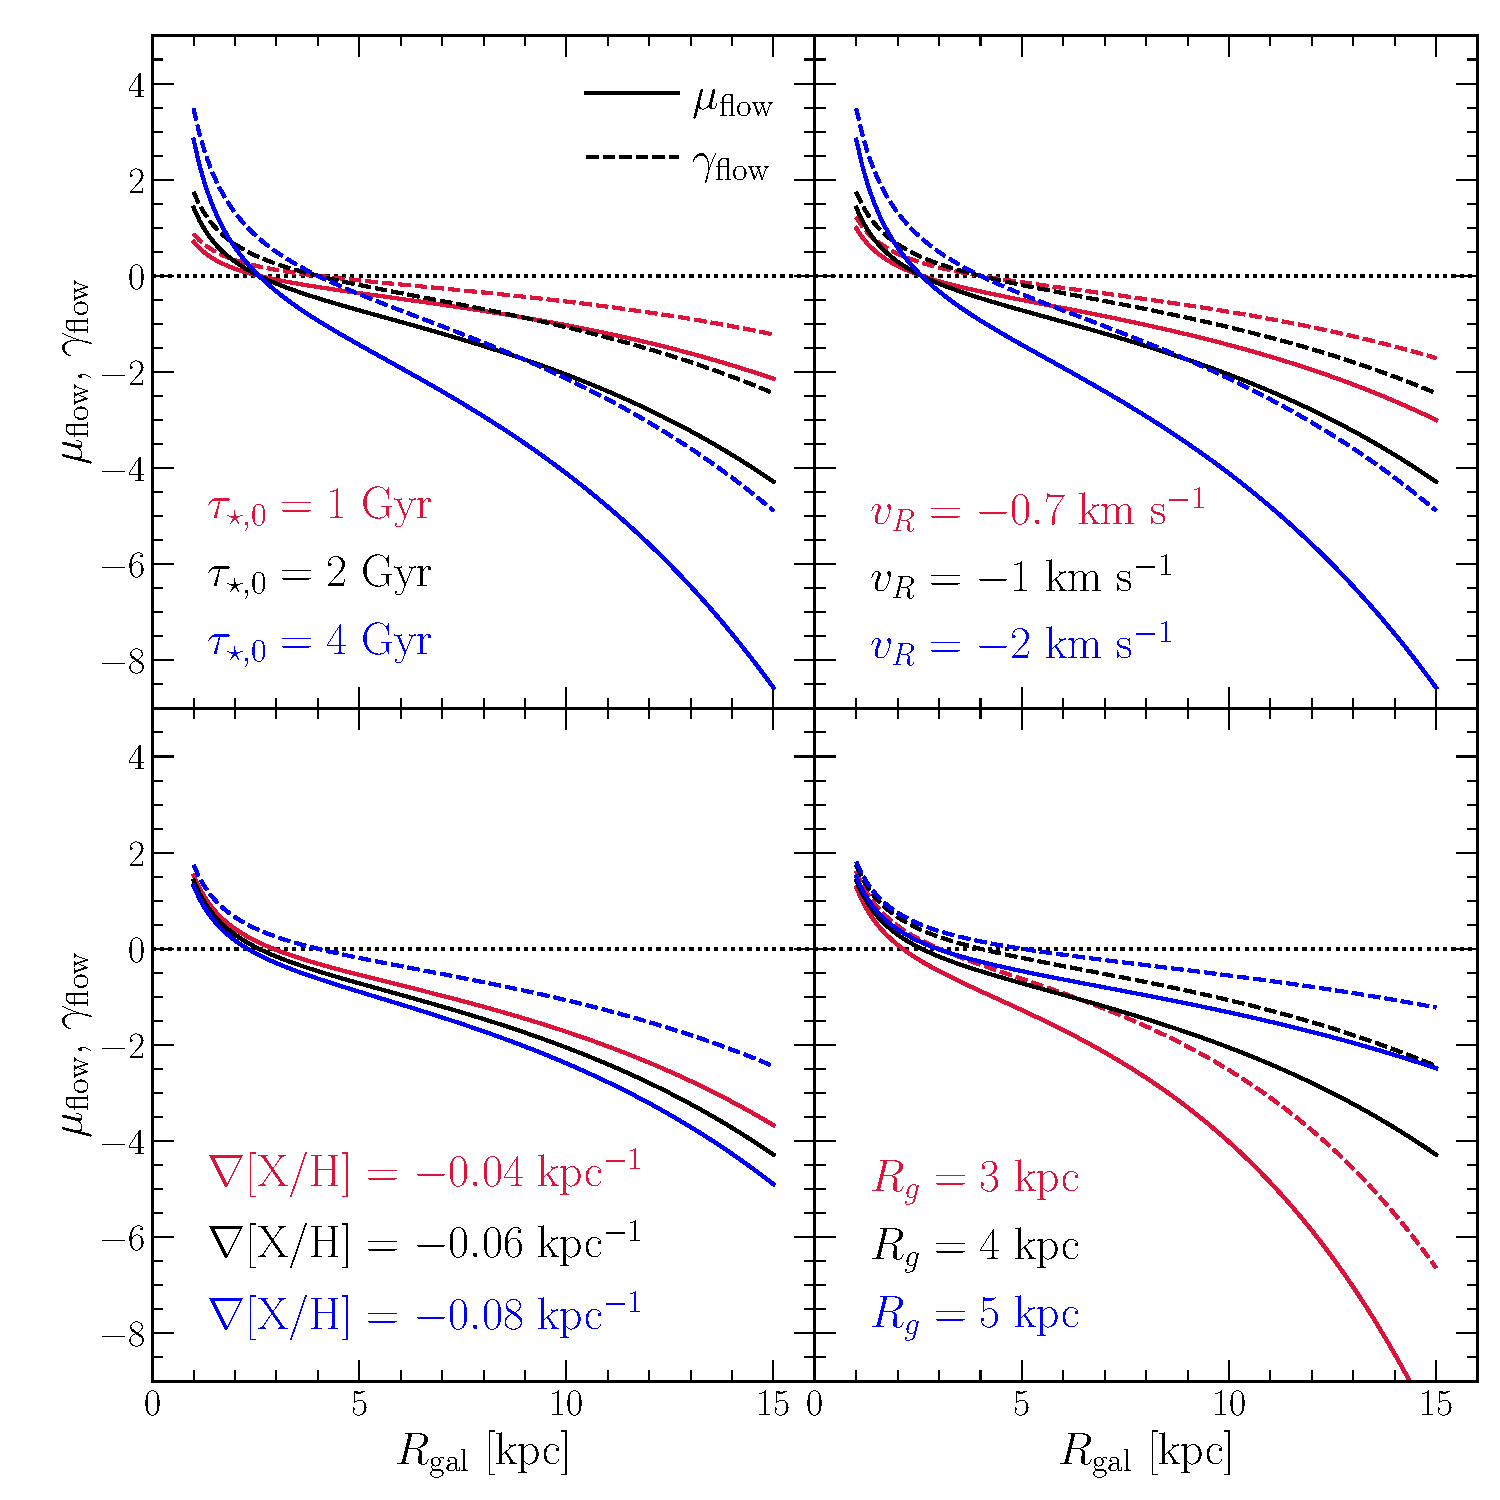
\includegraphics[scale = 0.5]{chapter7/muflow_gammaflow_vs_radius.pdf}
% \caption{
% The radial flow coefficients~$\mu_\flow$ (solid) and~$\gamma_\flow$ (dashed) as
% functions of radius for different parameter choices.
% Black lines correspond to the fiducial choice of
% ($\tau_{\star,0}$,~$v_g$,~\grad{X},~$R_g$) = (2 Gyr, 1 km s$^{-1}$,
% $-0.06$ kpc$^{-1}$,~$4$ kpc) and are the same in all panels.
% Each panel then shows variations in one of these four parameters according to
% the legends in the lower right.
% We also mark~$\mu_\flow$,~$\gamma_\flow = 0$ with a black dashed line, marking
% the boundary between a radial flow acting as a source versus a sink of metals
% and gas, respectively.
% }
% % \label{outflows:fig:flow-coefficients-vs-radius}
% \end{figure*}

% Fig.~\ref{outflows:fig:flow-coefficients-vs-radius} shows~$\mu_\flow$
% and~$\gamma_\flow$ as a function of radius for different parameter choices.
% By definition, radial flows are a~\textit{source} of metals when~$\mu_\flow > 0$
% and a~\textit{sink} when~$\mu_\flow < 0$; the same is true of the gas supply
% with~$\gamma_\flow$.
% In general, radial flows are a sink of both gas and metals across most of the
% Galactic disk, becoming a source term only at radii better associated with the
% bulge.
% We expect this result to be generic as the negative sign arises due to the
% difference between~$1 / R$, which varies, and~$1 / R_g + 1 / R_x$, which is
% constant for a given parameter selection.
% Flows are however a stronger sink for metals than gas under this
% parameterization since, by definition,~$\mu_\flow = \gamma_\flow + \tau_\star
% v_g / R_x$ and~$v_g < 0$.
% Both~$\tau_{\star,0}$ and~$v_g$ are normalizing factors on the flow
% coefficients, so they do not impact the radius at which~$\mu_\flow = 0$ or
% $\gamma_\flow = 0$, but increases in their values make flows a stronger sink
% where they are a sink and a stronger source where they are a source.
% Changes in the slopes of gradients, either metallicity or gas surface density,
% impact the flow rates in an intuitive manner: they are a stronger sink for more
% sharply declining gradients as the mass or metallicity at~$R + \Delta R$ is
% smaller in these cases.
% Interestingly, the exact slope of the metallicity gradient~\grad{X} has minimal
% impact on~$\mu_\flow$, potentially indicating that radial flows in turn have
% minimal impact on abundance gradients.

% \subsubsection{Analytic Solutions to Simple Cases}
% \label{outflows:sec:gce:onezone:analytic}
% Given a handful of simplifying assumptions, one-zone models often allow
% analytic solutions to the abundance by mass~$Z_x \equiv M_x / M_g$ as a
% function of time.
% Under the approximation that the SN Ia DTD is a simple exponential followed by
% some minimum delay,~\citet{Weinberg2017b} obtain solutions for~$Z_\text{O}$
% and~$Z_\text{Fe}$ within the formalism of equations~\refp{outflows:eq:mdot-gas}
% and~\refp{outflows:eq:mdot-element}.
% With the additional approximation that~$\mu_\flow$ is constant in time, which
% we expect to be accurate up to~$\sim$8 Gyr ago based on the results
% of~\S~\ref{outflows:sec:empirical}, the derivation proceeds similarly under the
% simple transformation~$1 + \eta - r \rightarrow 1 + \eta - r - \mu_\flow$.
% We briefly discuss this extension of the~\citet{Weinberg2017b} results here and
% refer readers to their~\S\S~2 and 3 for further details.
% \par
% The primary complication of the parameterization arises because
% $\mu_\flow \neq \gamma_\flow$.
% This inequality is a consequence of the radial metallicity gradient, which
% lowers the metallicity of inward flowing gas.
% % Fig.~\ref{outflows:fig:flow-coefficients-vs-radius} indicates that the amount
% % of mass lost from a given~$\Delta R$ annulus at Galactocentric radii outside of
% % the bulge over the course of some~$\Delta t$ timestep is replaced not only by
% % less gas, but lower metallicity gas.
% As a consequence, the~\textit{depletion time} of metals is shorter than that of
% the bulk gas.
% That is, in the absence of accretion (which would affect only the gas supply if
% it is zero metallicity), metals spend less time than non-metals within a given
% ISM fluid element before being incorporated into new stars or lost to an
% outflow or the radial flow.
% \par
% These timescales are defined as
% \begin{subequations}\begin{align}
% \timescale{dep,g} &\equiv \frac{M_g}{
% 	\dot{M}_\star + \dot{M}_\text{out} - \dot{M}_r - \dot{M}_{g,\flow}
% } = \frac{\tau_\star}{1 + \eta - r - \gamma_\flow}
% \\
% \timescale{dep,$x$} &\equiv \frac{M_x}{
% 	Z_x\left(\dot{M}_\star + \dot{M}_\text{out} - \dot{M}_r - \dot{M}_{x,\flow}
% 	\right)
% } = \frac{\tau_\star}{1 + \eta - r - \mu_\flow},
% \end{align}\end{subequations}
% and both reduce to the~\citet{Weinberg2017b} form
% $\timescale{dep} = \tau_\star / (1 + \eta - r)$ in the absence of a radial
% flow (i.e.,~$v_g = 0 \implies \mu_\flow = \gamma_\flow = 0$).
% In Appendix~\ref{outflows:sec:gce-supplement}, we demonstrate that their form
% of~\timescale{dep} should be replaced with the metal depletion time as opposed
% to the gas depletion time.
% % A generic expression for~$\dot{Z}_x$ can be derived by differentiating
% % $Z_x = M_x / (\dot{M}_\star \tau_\star)$ with time and substituting in
% % equation~\refp{outflows:eq:mdot-element-flow}, carrying~$\mu_\flow$ as opposed
% % to~$\gamma_\flow$ through the derivation.

% % {
% % \renewcommand{\arraystretch}{1.8}
% % \begin{table*}
% % \caption{
% % The SFHs we use in this analytic framework (left) and the implied functions of
% % time specifying the evolution toward chemical equilibrium (right; see equations
% % \ref{outflows:eq:z-o-eq} and~\ref{outflows:eq:fsfh-definition} and associated
% % discussion in~\S~\ref{outflows:sec:gce:onezone:analytic}).
% % }
% % \begin{tabularx}{\linewidth}{l @{\extracolsep{\fill}} r}
% % \hline
% % SFH Shape & $f_\text{sfh}$
% % \\
% % \hline
% % $e^{-t / \timescale{sfh}}$ &
% % $1 - e^{-t / \tau_\psi}$
% % \\
% % $te^{-t / \timescale{sfh}}$ &
% % $1 - \ddfrac{\tau_\psi}{t} \left(1 - e^{-t / \tau_\psi}\right)$
% % \\
% % $\left(1 - e^{-t / \timescale{rise}}\right) e^{-t / \timescale{sfh}}$ &
% % $\ddfrac{1}{1 - e^{-t / \timescale{rise}}} \left(
% % 1 - e^{-t / \tau_\psi} -
% % \ddfrac{\timescale{rise}}{\timescale{rise} - \tau_\psi}
% % \left(e^{-t / \timescale{rise}} - e^{-t / \tau_\psi}\right)
% % \right)$
% % \\
% % \hline
% % \end{tabularx}
% % \label{outflows:tab:f-sfh-forms}
% % \end{table*}
% % }

% As we are primarily interested in this analytic framework for qualitative
% interpretation, we focus this component of our investigation on O.
% This simplifies the parameterization as Fe abundances are additionally affected
% by SN Ia enrichment (see discussion in~\S~X.Y.Z below), and the expressions
% lend qualitative insight into the predicted Fe abundances anyway.
% Applying our transformation to the~\citet{Weinberg2017b} formalism results in
% the following expression for the equilibrium O abundance for the
% linear-exponential and pure exponential SFHs:
% \begin{equation}
% Z_{\text{O,eq}} =
% \frac{\ycc{O}}{1 + \eta - r - \mu_\flow - \tau_\star / \timescale{sfh}}.
% \label{outflows:eq:z-o-eq}
% \end{equation}
% In Appendix~\ref{outflows:sec:gce-supplement}, we demonstrate that the
% equilibrium abundance is the same for the ``inside-out'' SFH from
% Chapter~\ref{migration}.
% Of these three separate SFHs, the full time evolution of~$Z_x$ is given by
% \begin{equation}
% {Z}_\text{O}(t) = Z_\text{O,eq} f_\text{sfh}(t),
% % \label{outflows:eq:fsfh-definition}
% \end{equation}
% where~$f_\text{sfh}$ is some unitless function that depends on the SFH and
% specifies the detailed evolution toward equilibrium with time.
% Table~\ref{outflows:tab:f-sfh-forms} presents the time-dependence of these
% SFHs and the associated forms of~$f_\text{sfh}$, where the timescale~$\tau_\psi$
% is defined as 
% \begin{equation}
% \tau_\psi \equiv \left(
% \frac{1 + \eta - r - \mu_\flow}{\tau_\star} - \frac{1}{\timescale{sfh}}
% \right)^{-1}.
% % \label{outflows:eq:tau-psi-def}
% \end{equation}
% We also reserve the derivation of~$f_\text{sfh}$ for the inside-out SFH for
% Appendix~\ref{outflows:sec:gce-supplement}.

